\documentclass[../PhD_Dissertation.tex]{subfiles}
\begin{document}
\chapter{Introduction}{Introduction}
Insert introduction. \gls{eg} \cite{nmpc_book}:
\\\newline
\lipsum[2-4]
\\\newline
Figure \ref{fig: example_figure}
%%%%%%%%%%%%%%%%%%%%%%%%%%%%%%%%%%%%%%%%%%%%%%%%%
\begin{figure}[h]
  \centering
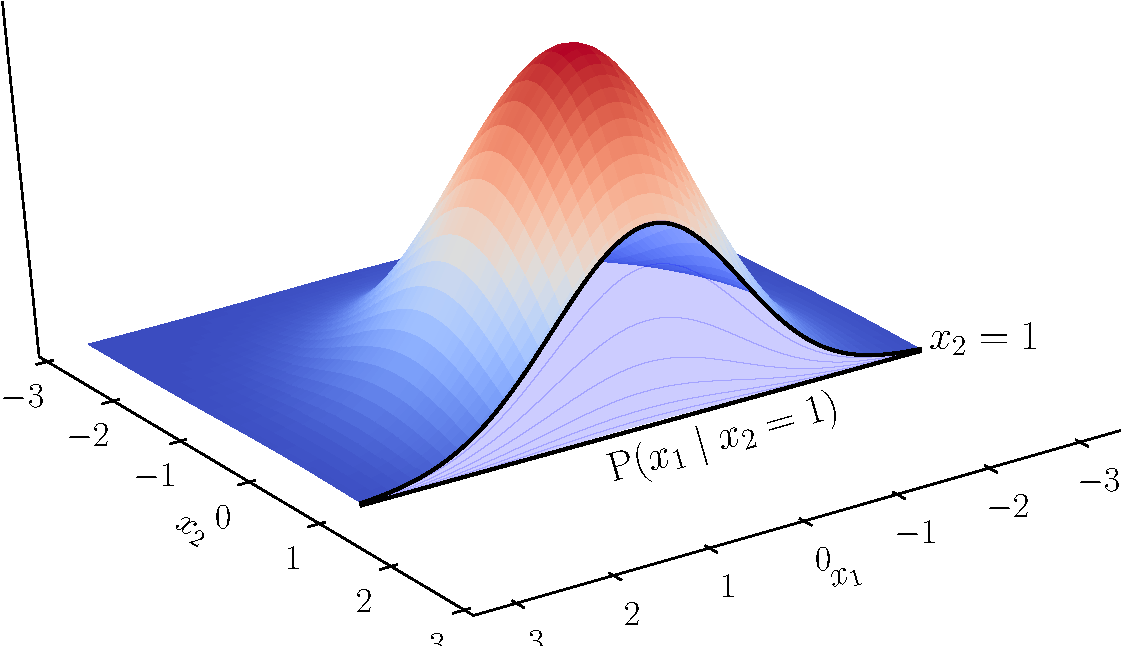
\includegraphics[width=0.75\textwidth]{Figures/conditional_gaussian.pdf}
  \caption{Example Figure} \label{fig: example_figure}
\end{figure}
\end{document}